\documentclass[../main]{subfiles}

\graphicspath{{../figures/}}

\begin{document}

\section{異常データを用いない移動ロボットを用いた異常音検知}
\label{sec:related_work_mobile}

移動ロボットにマイクを搭載し,搭載したマイクから得られる
音響信号をもとに異常音を検知する手法が存在する.
本研究では,この手法を移動ロボットを用いた異常音検知と呼ぶ.
移動ロボットを用いる場合,音の空間的な情報を取得することができるため,音源の位置推定にも頻繁に利用されている.
Songらは,機器の異常音を検出し,その異常音のパターンが最も大きくなる箇所を異常の位置として推定している\cite{9023943}.
しかし,Songらは,\reffig{fig:supervised_prev_research}に示すように,の周波数を取り出すためのフィルタをヒューリスティックに設計し,そのフィルタを用いて異常音を抽出している.
一方で,本研究において対象とする石油精製プラント内の異常は,前節で述べたように,傷の深さや位置によって異常音の周波数特性が異なるため,
Songらの手法をそのまま適用することは困難である.

次に,同様に移動ロボットを用いた異常音検知に関する研究としてFujitaらによる研究を紹介する\cite{10202270}.
Fujitaらは,\reffig{fig:fujita_previous_research}に示すように点検区域をグリッドに分割し,そのグリッド毎に正常音を学習し,各グリッド内で,そこで学習したモデルを用いて異常の有無を判別する手法を提案している.
この手法では,グリッドごとに異常音の有無を判定するため,異常音源が存在する区間を推定することが可能である.
しかし,グリッドの解像度でしか,異常を推定することができず,異常音源の位置の推定には至っていない.

以上で述べたように,移動ロボットを用いた異常音検知手法は,
異常音の前提知識が存在しない場合,異常音の位置推定が困難である.

\begin{figure}[t]
  \centering
  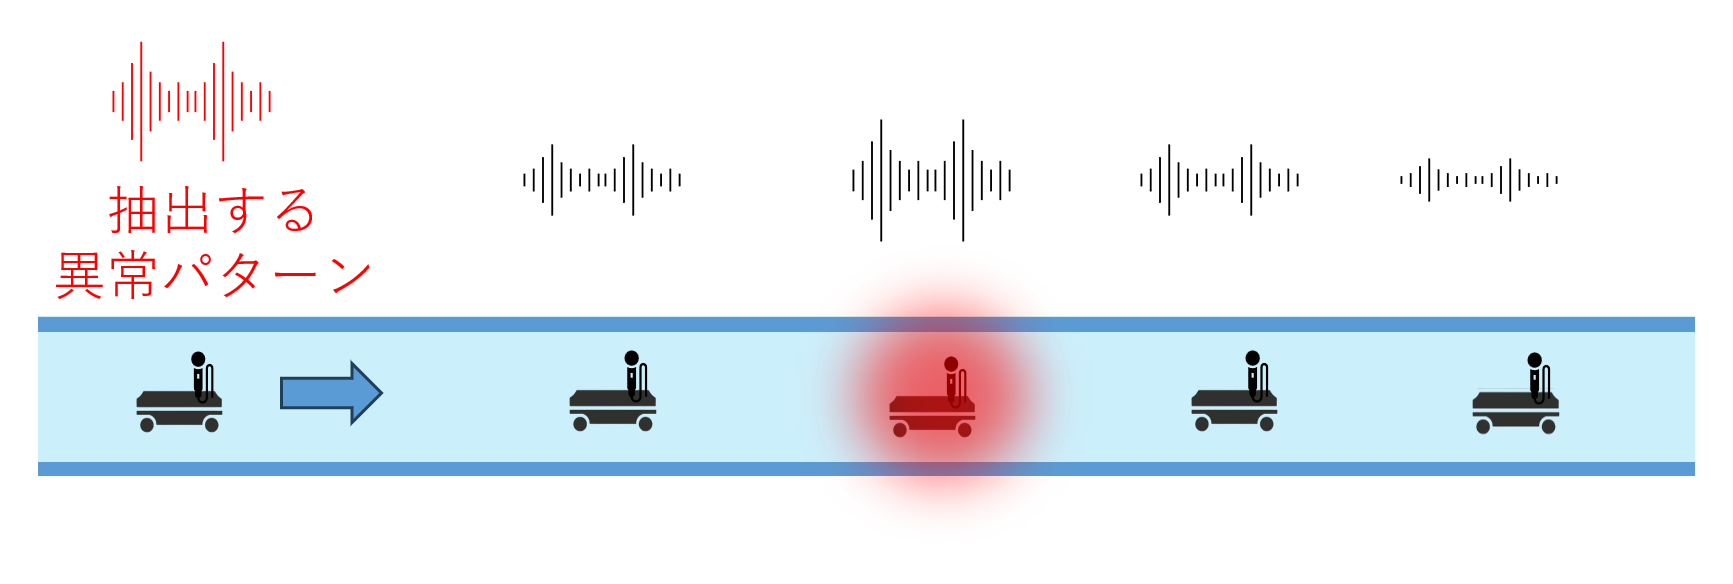
\includegraphics[keepaspectratio, width=1.0\linewidth]{chap2/supervised_prev_research.png}
  \caption{フィルタによる異常音抽出を用いた異常音検知の模式図}
  \label{fig:supervised_prev_research}
\end{figure}

\begin{figure}[t]
  \centering
  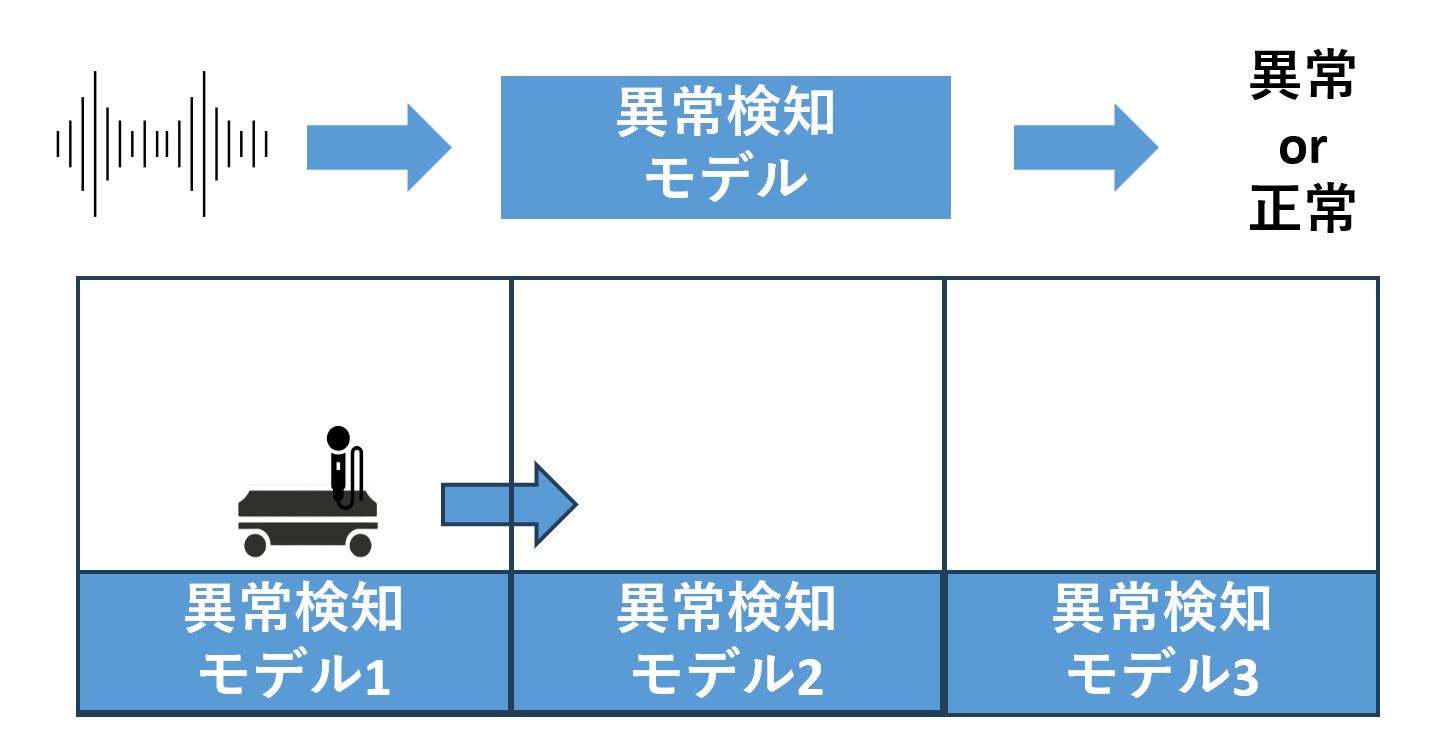
\includegraphics[keepaspectratio, width=1.0\linewidth]{chap2/fujita_previous_research.png}
  \caption{グリッド分割を用いた異常音検知の模式図}
  \label{fig:fujita_previous_research}
\end{figure}



\end{document}
